\chapter{PENDAHULUAN}
\label{chap:pendahuluan}

% Ubah bagian-bagian berikut dengan isi dari pendahuluan
\section{Latar Belakang}
\label{sec:latarbelakang}

Indonesia memiliki skor kriminalitas yang cukup tinggi di dunia pada tahun 2021. \linebreak
Berdasarkan data \emph{Criminal Scores} yang dibuat oleh \emph{Global Initiative Against Transnational Organized Crime} 
(GITOC), Indonesia tercatat memiliki skor 6.38 dan berada di urutan 25 dari 193 negara yang 
terdaftar di PBB \parencite{Gitoc2021}. Pada tahun 2020, angka kejahatan yang terjadi di Indonesia 
sebanyak 247.218 kasus dengan Sumatera Utara memiliki 32.990 kasus kejahatan \parencite{Bpskriminal2021}.
Beberapa kasus kejahatan yang terjadi sering menggunakan kendaraan sebagai alat untuk membantu pelaku 
dalam melaksanakan tindakannya.

Mobil yang digunakan di Indonesia diproduksi oleh merek dan perusahaan yang berbeda-beda 
dan setiap tipe yang diproduksi memiliki ciri khasnya masing-masing. Ciri khas ini dapat 
berupa bentuk badan kendaraan, jenis kendaraan, warna, serta ukuran. Ciri khas inilah 
yang dapat membantu mengidentifikasi tipe satu dengan lainnya.

\begin{figure}[ht]
      \centering
      % Nama dari file gambar yang diinputkan
      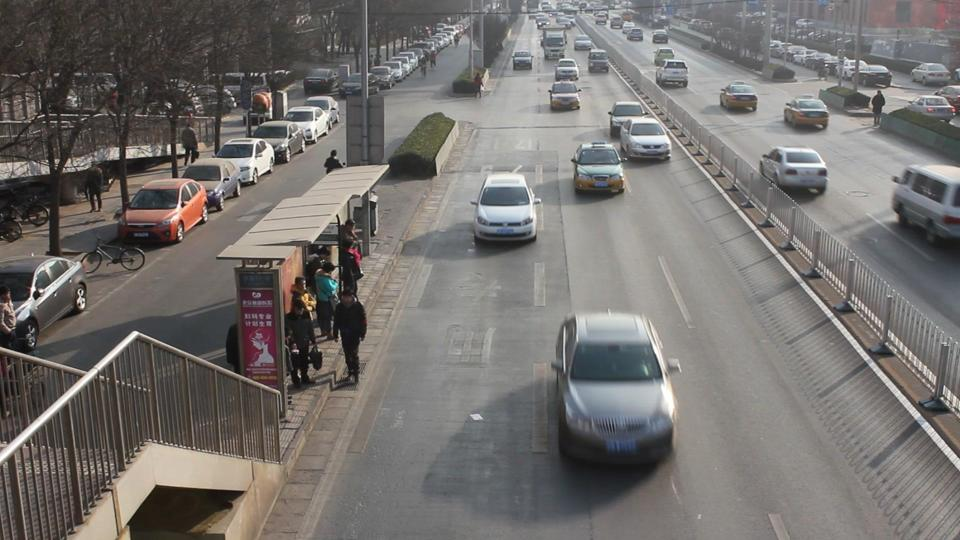
\includegraphics[scale=0.3]{gambar/Mobil.jpg}
      % Keterangan gambar yang diinputkan
      \caption{Lalu lintas dari rekaman CCTV}
      % Label referensi dari gambar yang diinputkan
      \label{fig:RekamanCCTV}
\end{figure}

Ciri khas yang dimiliki pada tiap tipe mobil inilah yang dapat membantu dalam melakukan 
re-identifikasi menggunakan metode Swin Transformer. Swin Transformer merupakan hasil 
pengembangan arsitektur Convolutional Neural Network (CNN) dan Vision Transformer yang 
baru. Swin Transformer memiliki kelebihan yang cukup menguntungkan jika dibandingkan 
dengan Vision Transformer, dimana Swin Transformer dapat memproses dan mengidentifikasi 
citra yang ditangkap dalam keadaan blur, resolusi yang kecil, dan pencahayaan yang tidak 
sempurna. Hasil yang diberikan oleh Swin Transformer lebih efisien dan akurasinya lebih tinggi.

Oleh karena itu, penulis merasa metode Swin Transformer dapat digunakan untuk membantu menangani 
kasus kejahatan. Dengan diaplikasikannya Swin Transformer pada tangkapan citra dari kamera pengawas 
lalu lintas, maka dapat mempermudah proses pemecahan kasus kejahatan dimana kendaraan yang digunakan 
pelaku dapat di re-identifikasi dan dilacak menggunakan tangkapan kamera pengawas lalu lintas di 
sekitar tempat kejadian perkara.

\section{Permasalahan}
\label{sec:permasalahan}

Dalam proses re-identifikasi mobil, sering kali terjadi kesalahan dalam melakukan re-identifikasi.
Gambar yang kurang jelas karena dalam kondisi lingkungan dengan pencahayaan yang tidak ideal,
resolusi dari gambar yang cukup kecil, serta adanya blur ketika proses pengambilan gambar, membuat model re-identifikasi
yang sudah ada saat ini belum bisa melakukan re-identifikasi mobil secara maksimal menggunakan 
tangkapan citra dari kamera pengawas lalu lintas.

\section{Batasan Masalah}
\label{sec:batasanmasalah}

Batasan-batasan permasalah yang diangkat pada penelitian ini berdasarkan permasalahan diatas adalah:

\begin{enumerate}[nolistsep]

      \item Pengembangan model re-identifikasi hanya berfokus pada kendaraan mobil dan roda empat sebagai objek

      \item Model re-identifikasi yang dibuat menggunakan Metode Swin Transformer dari \emph{Pytorch 
      ReID layumi} 

      \item Dataset yang digunakan merupakan dataset mobil yang sudah memiliki pemisahan yaitu \emph{VRIC}
      (\emph{Vehicle Re-Identification in Context})

      \item Penulis hanya melakukan pengembangan model re-identifikasi menggunakan \emph{Swin Transformer} dan tidak 
      mengembangkan sistem secara keseluruhan

\end{enumerate}

\section{Tujuan}
\label{sec:Tujuan}

Dari permasalahan yang telah dituliskan diatas dapat dikatakan bahwa re-identifikasi mobil belum maksimal
ketika dihadapkan pada kondisi-kondisi tertentu, sehingga tujuan dari penelitian ini adalah untuk membuat
sebuah sistem re-identifikasi mobil menggunakan bentuk arsitektur terbaru Vision Transformer yaitu 
Swin Transformer agar dapat mengidentifikasi ulang mobil ketika dihadapkan pada kondisi-kondisi tertentu.

\section{Manfaat}
\label{sec:manfaat}

Manfaat dari penelitian adalah :

\begin{enumerate}[nolistsep]
  
  \item Bagi penulis
  
  Seluruh proses yang dijalani penulis dalam pelaksanaan pengerjaan Tugas Akhir
  kali ini memberikan banyak manfaat kepada penulis, antara lain seperti mengasah
  kemampuan untuk pemecahan permasalahan nyata yang dihadapi oleh masyarakat,
  pola pikir yang kritis, logis dan sistematis dalam perumusan sintesis pemecahan
  masalah, keterampilan dalam menyusun laporan pengerjaan Tugas Akhir, dll.
  \item Bagi institusi
  
  Melalui laporan Tugas Akhir ini, penulis berharap dapat memberikan inspirasi dan
  referensi terkait inovasi - inovasi dalam bidang \emph{Deep Learning} menggunakan 
  metode terbarunya. Sehingga perancangan ini tidak berhenti sampai disini saja.
  \item Bagi masyarakat
  
  Penulis berharap bahwa pengerjaan Tugas Akhir ini dapat menjadi sebuah solusi yang 
  tepat untuk penyelesaian dari sebuah aspek permasalahan
  maupun kebutuhan masyarakat sehingga dapat memberikan manfaat yang nyata.
  Dan secara khusus untuk penyelidikan yang dilakukan polisi diharap model re-identifikasi yang dibuat
  dapat membantu dalam pemecahan kasus kejahatan.
  
\end{enumerate}

% \section{Sistematika Penulisan}
% \label{sec:sistematikapenulisan}

% Laporan penelitian tugas akhir ini terbagi menjadi \lipsum[1][1-3] yaitu:

% \begin{enumerate}[nolistsep]

%   \item \textbf{BAB I Pendahuluan}

%         Bab ini berisi \lipsum[2][1-5]

%         \vspace{2ex}

%   \item \textbf{BAB II Tinjauan Pustaka}

%         Bab ini berisi \lipsum[3][1-5]

%         \vspace{2ex}

%   \item \textbf{BAB III Desain dan Implementasi Sistem}

%         Bab ini berisi \lipsum[4][1-5]

%         \vspace{2ex}

%   \item \textbf{BAB IV Pengujian dan Analisa}

%         Bab ini berisi \lipsum[5][1-5]

%         \vspace{2ex}

%   \item \textbf{BAB V Penutup}

%         Bab ini berisi \lipsum[6][1-5]

% \end{enumerate}
